\section{Durchführung}
\label{sec:Durchführung}

\subsection{Vorbereitungsaufgaben}
\label{sec:vorbereitung}
In folgender Tabelle sind die recherchierten Werte für den Brechungsindex verschiedener Materialien zusammengefasst:
\begin{table}[H]
  \centering
  \caption{Brechungsindizes verschiedener Materialien.}
  \label{tab:brechungsind}
  \sisetup{table-format=1.8}
  \begin{tabular}{S S}
    \toprule
    {Material} & {$n$} \\
    \midrule
    {Luft}            & 1.00029317 \\
    {Wasser}          & 1.344661 \\
    {Borkron K1}      & 1.51201 \\
    {Schwerkron SK1}  & 1.61282 \\
    {Plexiglas}       & 1.4931 \\
    {Diamant}         & 2.4235 \\
    \bottomrule
  \end{tabular}
\end{table}

\noindent
Die berechneten Gitterkonstanten werden im Folgenden angegeben:
\\
Für $600$ Linien/$\si{\milli\meter}$ gilt

\begin{equation}
  d = \frac{1}{600} \si{\milli\meter}.
\end{equation}
\noindent

Für $300$ Linien/$\si{\milli\meter}$ gilt

\begin{equation}
  d = \frac{1}{300} \si{\milli\meter}.
\end{equation}
\noindent

Für $100$ Linien/$\si{\milli\meter}$ gilt

\begin{equation}
  d = \frac{1}{100} \si{\milli\meter}.
\end{equation}
\noindent

\subsection{Versuchsaufbau}
\label{sec:aufbau}
Der Versuchsaufbau besteht aus einer transparenten Platte, auf welcher sich ein roter
($\lambda=\SI{635}{\nano\metre}$) und ein grüner ($\lambda=\SI{532}{\nano\metre}$) Laser
befinden. Die Laser lassen sich dabei im Halbkreis um die Platte bewegen, sodass verschiedene
Winkel eingestellt werden können. Diese können dann an der Skala auf der Platte abgelesen werden.
Um die Experimentierenden vor dem Laserlicht zu schützen ist zudem noch ein Reflexionsschirm
verbaut. Diese Apparatur ist in Abbildung \ref{fig:Aufbau} dargestellt.
\\\noindent
In der Mitte der Apparatur \ref{fig:Aufbau} lassen sich nun optische Elemente positionieren, welche
in Abbildung \ref{fig:Teile} dargestellt sind.
\begin{figure}[H]
    \centering
    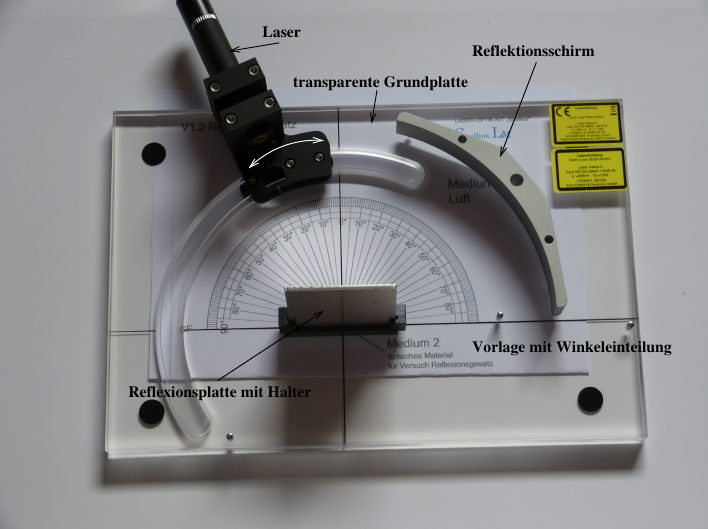
\includegraphics[scale = 0.3]{pictures/Aufbau.png}
    \caption{Die Versuchsapparatur. Quelle: \cite{AP01}}
    \label{fig:Aufbau}
\end{figure}
\begin{figure}[H]
    \centering
    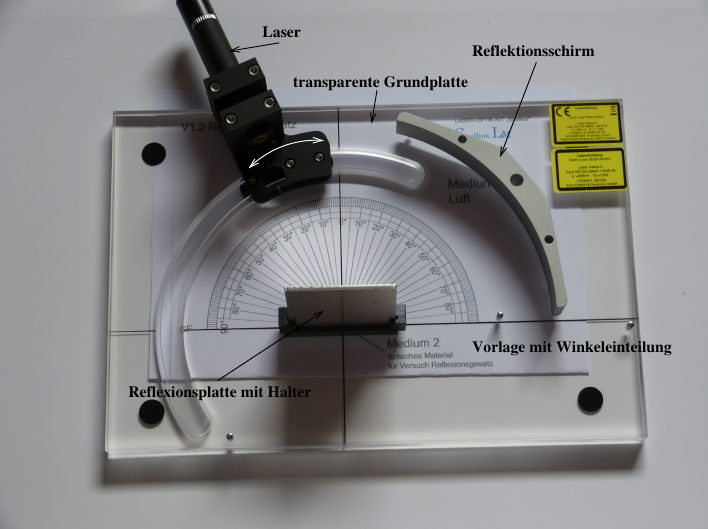
\includegraphics[scale = 0.3]{pictures/Teile.png}
    \caption{Optische Elemente. Quelle: \cite{AP01}}
    \label{fig:Teile}
\end{figure}


\subsection{Reflexionsgesetz}
\label{sec:reflexionsmessung}
\subsection{Brechungsgestz}
\label{sec:brechungmessung}
\subsection{Strahlenversatz}
\label{sec:strahlenversatzmessung}
\subsection{Prisma}
\label{sec:prismamessung}
